\section{Geometric Meaning of Vector Addition}

\begin{outcome}

\begin{enumerate}
\item[A.] Understand vector addition, geometrically.
\end{enumerate}
\end{outcome}

Recall that an element of $\mathbb{R}^{n}$ is an ordered list of
numbers. For the specific case of $n=2,3$ this can be used to
determine a point in two or three dimensional space. This point is
specified relative to some coordinate axes.

Consider the case $n=3$. Recall that taking a vector and moving it
around without changing its length or direction does not change the
vector. This is important in the geometric representation of vector
addition.

Suppose we have two vectors, $\vect{u}$ and $\vect{v}$ in
$\mathbb{R}^{3}$. Each of these can be drawn geometrically by placing
the tail of each vector at $0$ and its point at $\left( u_{1}, u_{2},
u_{3}\right)$ and $\left( v_{1}, v_{2}, v_{3}\right) $
respectively. Suppose we slide the vector $\vect{v}$ so that its tail
sits at the point of $\vect{u}$.  We know that this does not change
the vector $\vect{v}$.  Now, draw a new vector from the tail of
$\vect{u}$ to the point of $\vect{v}$. This vector is
$\vect{u}+\vect{v}$.

The geometric significance of vector addition in $\mathbb{R}^n$ for any $n$ is given in
the following definition.

\begin{definition}{Geometry of Vector Addition}{geometryofvectoraddition}
Let $\vect{u}$ and $\vect{v}$ be two vectors. Slide $\vect{v}$ so that
the tail of $\vect{v}$ is on the point of $\vect{u}$. Then draw the
arrow which goes from the tail of $\vect{u}$ to the point of $\vect{v}$. 
This arrow represents the vector $\vect{u}+\vect{v}$.

\begin{center}
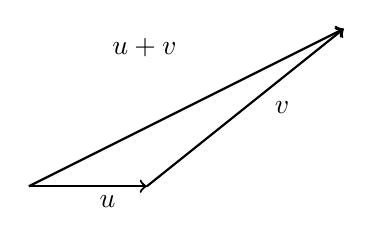
\begin{tikzpicture}[scale=2]
\draw[->, thick](0,0)--(2,1);
\draw[->, thick](0,0)--(0.75,0);
\draw[->, thick](0.75,0)--(2,1);
\node[below left] at (1,1){$\vect{u}+\vect{v}$};
\node[below] at (0.5,0){$\vect{u}$};
\node[right] at (1.5,0.5){$\vect{v}$};
\end{tikzpicture}
\end{center}
\end{definition}

This definition is illustrated in the following picture in which
$\vect{u}+\vect{v}$ is shown for the special case $n=3$.

\begin{picture}(1,190)
\put(120,40){\begin{picture}(1,1) %\thicklines
\setlength{\unitlength}{1pt} \put(0,0){\line(-1,-1){30}}
\put(0,0){\line(0,1){50}}\put(0,0){\line(1,0){80}}
\put(20,80){\put(0,0){\vector(1,1){40}} \qbezier[20](40,40)(40,10)(40,-20)
  \qbezier[10](40,-20)(50,-10)(60,0)
  \qbezier[20](40,-20)(10,-20)(-20,-20)
  \qbezier[10](-20,-20)(-10,-10)(0,0)
  \qbezier[20](0,0)(30,0)(60,0)
  \qbezier[15](0,0)(0,20)(0,40)\put(20,25){$\vect{v}$}}
  \put(0,0){\put(0,0){\vector(1,4){20}}}
  \put(5,50){$\vect{u}$}\put(0,0){\vector(1,2){60}}\put(60,45){$\vect{u}+\vect{v}$}
  \put(55,50){\vector(-1,1){20}}
 \put(0,0){\put(0,0){\vector(1,1){40}} \qbezier[20](40,40)(40,10)(40,-20)
  \qbezier[10](40,-20)(50,-10)(60,0)
  \qbezier[20](40,-20)(10,-20)(-20,-20)
  \qbezier[10](-20,-20)(-10,-10)(0,0)
  \qbezier[20](0,0)(30,0)(60,0)
  \qbezier[15](0,0)(0,20)(0,40)
  \put(22,15){$\vect{v}$}}
  \put(-35,-25){$x$}
  \put(-10,45){$z$}
  \put(75,3){$y$}
  \put(40,40){\qbezier[15](0,0)(10,40)(20,80)}
\end{picture}}
\end{picture}

Notice the parallelogram created by $\vect{u}$ and $\vect{v}$ in the above diagram. 
Then $\vect{u} + \vect{v}$ is the directed
diagonal of the parallelogram determined by the two vectors $\vect{u}$ and
$\vect{v}$.

When you have a vector $\vect{v}$, its additive inverse $-\vect{v}$ will
be the vector which has the same magnitude as $\vect{v}$ but the opposite
direction. When one writes $\vect{u}-\vect{v,}$ the meaning is $\vect{u} + \left(
-\vect{v}\right) $ as with real numbers. The following example illustrates these definitions and conventions.

\begin{example}{Graphing Vector Addition}{graphingvectoraddition}
Consider the following picture of vectors $\vect{u}$ and $\vect{v}$.

\begin{center}
\begin{tikzpicture}[scale=2]
\draw[->, thick, blue] (0,0)--(2,1);
\draw[->, thick, red] (4,1)--(5,0.5);
\node[below] at (1,1.25){$\vect{u}$};
\node[above right] at (4.5, 0.75){$\vect{v}$};
\end{tikzpicture}
\end{center}

Sketch a picture of $\vect{u}+\vect{v},\vect{u}-\vect{v}.$
\end{example}

\begin{solution}
We will first sketch $\vect{u}+\vect{v}.$ Begin by drawing $\vect{u}$
and then at the point of $\vect{u}$, place the tail of $\vect{v}$ as
shown. Then $\vect{u}+\vect{v}$ is the vector which results from
drawing a vector from the tail of $\vect{u}$ to the tip of $\vect{v}$.

\begin{center}
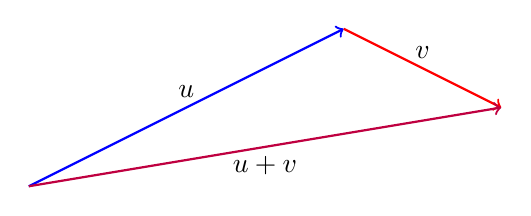
\begin{tikzpicture}[scale=2]
\draw[->, thick, blue](0,0)--(2,1);
\draw[->, thick, red](2,1)--(3,0.5);
\draw[->, thick, purple](0,0)--(3,0.5);
\node[above] at (1,0.5){$\vect{u}$};
\node[above] at (2.5, 0.75){$\vect{v}$};
\node[below] at (1.5, 0.25){$\vect{u}+\vect{v}$};
\end{tikzpicture}
\end{center}

Next consider $\vect{u}-\vect{v}.$ This means $\vect{u}+\left( -\vect{v}
\right) .$ From the above geometric description of vector addition, $-\vect{v}$ 
is the vector which has the same length but which points in the
opposite direction to $\vect{v}$. Here is a picture.

\begin{center}
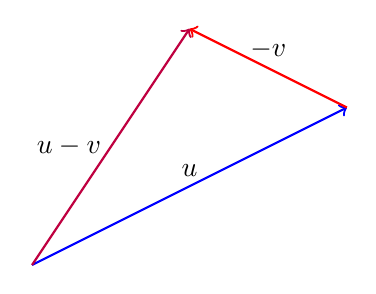
\begin{tikzpicture}[scale=2]
\draw[->, thick, blue](0,0)--(2,1);
\draw[->, thick, red](2,1)--(1,1.5);
\draw[->, thick, purple](0,0)--(1,1.5);
\node[above] at (1,0.5){$\vect{u}$};
\node[above] at (1.5, 1.25){$-\vect{v}$};
\node[left] at (0.5, 0.75){$\vect{u}-\vect{v}$};
\end{tikzpicture}
\end{center}
\end{solution}